
\chapter{METHODOLOGY/MODEL EQUATION}


\section{{\bf{Conceptual Framework - Truss}}}
    Truss is a structure consisting of organized objects in a shape of connecting triangles in such a way that it behaves as a single unit object. In order to enable the distribution of weight and grasp up the the fluctuating tension and compression without bending and shearing, it is made up of a web of triangles which is most stable form of geometry. In general, truss is used since it has a long life span and has least weight to the possible which in turn supports large loads and reduces deflections.\\

Commonly used in bridges, roofs and high rise buildings, it gives high value for mega constructions like the Eiffel Tower, construction of a stadium and all. We can think of truss as a beam where the web consists of series of separate members instead of a continuous plate. In engineering perspective, a truss is a structure that comprises of one or more triangular units constructed in a linear pattern such that its ends are connected to joints which is called as external nodes. The external forces and reaction to the forces are considered to act only at the nodes and the results in forces in the members are either tensile or compressive forces. In truss, the lower horizontal structure and the upper horizontal structure carry tension and compression. The diagonal and vertical structure form the truss web and it carries shear stress. Technically, they are also in tension and compression where the exact arrangement of forces depends on the type of truss and on the direction of bending. The structures serves in order to stabilize each other in order to prevent buckling. The structures that are under compression are to be designed to be safe against buckling. After knowing the force on each member, we determine the cross sectional area of the individual truss members. The weight of truss structure depends directly on its cross section area. The effect of weight of individual structures in a large truss is generally insignificant compared to the force exerted by external loads.\\

Later, after determining the minimum area of cross section of individual structures, it is dealt with bolted joints that involves shear stress of the bolt and connections used in the joints. The joints of truss can be designed as rigid, semi-rigid, or hinged.\\

Equation of truss: \\

The strain-displacement relationship is: \\
\begin{eqnarray}
	\epsilon = \frac{du}{dx}\\
	\sigma = E\epsilon
\end{eqnarray}

From the law of equilibruim, we get,
\begin{eqnarray}
	A\sigma_x = T = constant
\end{eqnarray}

Combining, the equations, we get:
\begin{eqnarray}
	AE\frac{du}{dx} = T = constant
\end{eqnarray}

Differentiating with respect to x, we get,
\begin{eqnarray}
	\frac{d}{dx}(AE\frac{du}{dx}) = 0
\end{eqnarray}
is the equation of truss.

%   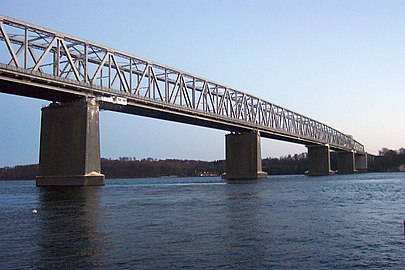
\includegraphics{3}\\
Fig:  Truss in bridge\\

%   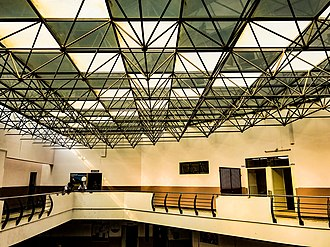
\includegraphics{2}\\
Fig:  Truss in roofing\\

%   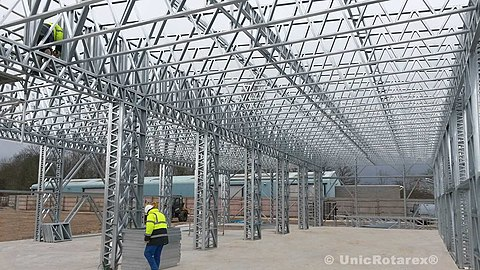
\includegraphics{5}\\
Fig: Three Dimensional Truss\\




\section{\bf{Mathematical Model and solution methods}}
{\bf\color{red}In this section, the author(s) should describe the theoretical/mathematical principles behind the whole work relative to the project. The information collected from literature review shall be relevant in this section.
}
%part assigned to samrajya

Consider\\
\begin{eqnarray}
	-\frac{d}{dx} \left[a(x)\frac{du}{dx} \right] = f(x)  \quad\quad  \text{for} \quad\quad  0<x<L.\\
\end{eqnarray}
for $u(x)$ subject to the boundary conditions\\
\begin{eqnarray}
	u(0)= u_0 \\
	\vspace{1cm}
	a(x)\frac{du}{dx}\biggr|_{x=L} = Q_L	
\end{eqnarray}
where $a(x)$ and $f(x)$ are known functions and 
$u_0$ and $Q_L$ are known values.
In case of bar (which is a axially loaded structure)\\

\begin{eqnarray*}
	u = \text{displacement}\\
	a(x)= \text{EA (stiffness)}\\
	f = \text{distributed axial force}\\
	Q_L= \text{axial load}\\
\end{eqnarray*}

Now, we want an approximation of u(x) in the form
\begin{eqnarray}
	u(x)\approx u_N(x) = \sum\limits_{j=1}^N c_j\phi_{j} + (x) +\phi_{0}(x)
\end{eqnarray}

%%page 2 of copy

 Substituting  $U_N$(x) in our Differential Equation,\\
 
 \begin{eqnarray}
 	-\frac{d}{dx} \left[a(x)\frac{dU_N}{dx} \right] = f(x)  \quad\quad  \text{for} \quad\quad  0<x<L.
 \end{eqnarray}

If this equally holds for all $x \in [0,L] $ the solution is exact. Since, we assume it only as an approximation.
we define Residual Function $R(x,c_1, c_2, c_3,...,c_N)$ as
\begin{eqnarray}
	R = -\frac{d}{dx} \left[a(x)\frac{dU_N}{dx} \right] - f(x)
\end{eqnarray} 

We have R $\neq$0 $ \forall x  \in [0, L]$  as a $U_N$ is only a approximation to solution.\\

Now we have various ways to minimize R in some senses over the domain to make this approximation close to the actual solution\\
\begin{enumerate}
	\item Collocation Method\\
	It forces that R is zero at selected N points of the domain.\\
	i.e; 
	\begin{eqnarray}
		R(x,c_1, c_2, c_3,...,c_N) = 0  \quad\quad\quad \forall x=x_i, i = 1,2,...,N
	\end{eqnarray}

	\item Least Square Method
		\begin{eqnarray}
			\frac{\partial}{\partial c_j} \int_{0}^{L} R^2 dx = 0 \quad\quad\quad \forall i = 1,2,...,N
		\end{eqnarray}
	
	\item Weighted Residual Method
		we desire that 
			\begin{eqnarray}
				\int_{0}^{L} w_i(x) R dx = 0 \quad\quad\quad \forall i = 1,2,...,N
			\end{eqnarray}
		where $w_i(x)$ are N linearly independent functions called weight functions.
\end{enumerate}

%page 4
	Now we convert our differential equation and boundary condition to weak form.\\
\begin{itemize}
	\item Step 1 : \\
	We write the weighted integral statement, i.e;\\
	\begin{eqnarray}
		\int_{0}^{L}  w \left[ -\frac{d}{dx} \left( a(x)\frac{du}{dx} \right) - f \right] dx = 0
	\end{eqnarray}

	It is equivalent to differential equations and does not include any boundary conditions and thus the variable $u$ must be differentiable to as many order as is required by the differential equation.
	\item Step 2\\
	Weakening Differentiability conditions
	\begin{eqnarray}
		\int_{0}^{L}  \left( w \left[ -\frac{d}{dx} \left( a(x)\frac{du}{dx} \right) \right] - wf \right)  dx = 0
	\end{eqnarray}
	Integrating by parts, we get,
	\begin{eqnarray}
		\int_{0}^{L} \left[ a \frac{dw}{dx} \frac{du}{dx} - wf \right] dx  - \left[ wa \frac{du}{dx}\right]_0^L = 0
	\end{eqnarray}

%%page 5 of copy

	we have used the fact that 
	\begin{eqnarray}
		\int_{a}^{b} \left( w \frac{dv}{dx} \right)dx  =  -\int_{a}^{b} v dw + \left[wv\right]_0^L = 0
	\end{eqnarray}

by considering,
	\begin{eqnarray}
		v = -a\frac{du}{dx}
	\end{eqnarray}

we can see that now we require that w be differentiable at least once but this also made that u needs to be differentiable only once even though the equation is of second order.//
Now, we take care of the boundary conditions which are of two types
\begin{itemize}
	\item Natural Boundary  condition
	\item Essential Boundary Condition 
\end{itemize}

Before defining these conditions we define primary and secondary variables.

\begin{df}{Primary Variable}
	pass
\end{df}
\begin{df}{Secondary Variable}
	pass
\end{df}

In our case , $ a \frac{du}{dx}$ is secondary variable.

If secondary variable(SV) is specified in the boundary, then such conditions are called natural boundary conditions (NBC).
If primary variable(PV) is specified in the boundary, then such conditions are called essential boundary conditions (NBC).

let us now define secondary variable as Q.
\begin{eqnarray}
	Q = a\frac{du}{dx} n_x
\end{eqnarray}

where $n_x$ is ???

For 1D problems,

\begin{eqnarray}
	n_x = -1 \quad\quad\quad \text{at left}\\
	n_x = 1 \quad\quad\quad \text{at right}
\end{eqnarray}

%Page 7 from copy

	\begin{eqnarray}
	\int_{0}^{L} \left[ a \frac{dw}{dx} \frac{du}{dx} - wf \right] dx  - \left[ wa \frac{du}{dx}\right]_0^L = 0
    \end{eqnarray}
	$\implies$
	\begin{eqnarray}
		\int_{0}^{L} \left[ a \frac{dw}{dx} \frac{du}{dx} - wf \right] dx  + wa\frac{du}{dx}\biggr|_{x=L} - wa\frac{du}{dx}\biggr|_{x=0} = 0
	\end{eqnarray}
	since $n_x = -1 \text{at} x = 0 $ and $n_x = 1 \text{at} x = L$
	\begin{eqnarray}
		\int_{0}^{L} \left[ a \frac{dw}{dx} \frac{du}{dx} - wf \right] dx  - n_xwa\frac{du}{dx}\biggr|_{x=L} - n_xwa\frac{du}{dx}\biggr|_{x=0} = 0
	\end{eqnarray}
	\begin{eqnarray}
	\int_{0}^{L} \left[ a \frac{dw}{dx} \frac{du}{dx} - wf \right] dx  -(wQ)_0  -(wQ)_L = 0
	\end{eqnarray}
	
	Finally we require that weight functions vanishes at boundaries where essential boundary conditions are specified.
	\begin{eqnarray}
		u(0) = u_0 \implies w(0) = 0
	\end{eqnarray}
Thus, we get
	\begin{eqnarray}
		\int_{0}^{L} \left[ a \frac{dw}{dx} \frac{du}{dx} - wf \right] dx   -w(L)Q_L = 0
	\end{eqnarray}

	
\end{itemize}
%part after assigning to samrajya

\begin{eqnarray}
	B(w,u) = \int_{0}^{L} a \frac{dw}{dx} \frac{du}{dx} dx \\
	l(w) = \int_{0}^{L} wf dx + w(L) Q_L
\end{eqnarray}

Hence, our weak form can be written as

\begin{eqnarray}
	0 = B(w,u) - l(w)
\end{eqnarray}
or ,
\begin{eqnarray}
	B(w,u) = l(w)
\end{eqnarray}

This is the variational form of the problem that is associated with our ODE and its boundary conditions.

When the differential equation is linear and of even order, the resulting weak form will have symmetric bi-linear form in u and w.
 	

% Choosing approximate functions

Let us now choose the approximate solutions that satisfy the two conditions for primary variables as other conditions are already included in the weak form. 
i.e,

\begin{eqnarray}
	u_h^{e} (x_a) = u_1^{e} \\
	u_h^{e} (x_b) = u_2^{e}  
\end{eqnarray}
let,
\begin{eqnarray}
	u_h^{e} (x) = c_1 + c_2 x
\end{eqnarray}

Then by the conditions,

\begin{eqnarray}
	u_h^{e} (x_a) = c_1 + c_2 x_a = u_1^{e}\\
	u_h^{e} (x_b) = c_1 + c_2 x_b = u_2^{e}
\end{eqnarray}

writing in matrix form, we obtain
\begin{eqnarray}
\begin{bmatrix}
	u_1^{e}\\
	u_2^{e}
\end{bmatrix}
=
\begin{bmatrix}
	1 & x_a\\
	1 & x_b
\end{bmatrix}
\begin{bmatrix}
	c_1^{e}\\
	c_2^{e}
\end{bmatrix}
\end{eqnarray}

We can rewrite the equations as 
\begin{eqnarray}
	\begin{bmatrix}
		c_1^{e}\\
		c_2^{e}
	\end{bmatrix}
	= \frac{1}{x_b - x_a}
	\begin{bmatrix}
		x_b & -x_a\\
		-1 & 1
	\end{bmatrix}
	\begin{bmatrix}
		u_1^{e}\\
		u_2^{e}
	\end{bmatrix}
\end{eqnarray}

Hence we get,

\begin{eqnarray}
	c_1^{e} = \frac{1}{h_e} (x_bu_1^e - x_bu_2^e)
\end{eqnarray}
\begin{eqnarray}
	c_2^{e} = \frac{1}{h_e} (-u_1^e + u_2^e)
\end{eqnarray}

If we let,
\begin{eqnarray*}
	\alpha_1^e = x_b\\
	\alpha_2^e = - x_a\\
	\beta_1^e = -1 \\
	\beta_2^e = 1	
\end{eqnarray*}

\begin{eqnarray}
	c_1^{e} = \frac{1}{h_e} (\alpha_1^e u_1^e + \alpha_2^e u_2^e)
\end{eqnarray}
\begin{eqnarray}
	c_2^{e} = \frac{1}{h_e} (\beta_1^eu_1^e + \beta_2^e u_2^e)
\end{eqnarray}

Hence,
\begin{eqnarray*}
	U_h^e(x) =  \frac{1}{h_e} [\alpha_1^e u_1^e + \alpha_2^e u_2^e + (\beta_1^eu_1^e + \beta_2^e u_2^e)x]
\end{eqnarray*}
\begin{eqnarray*}
	U_h^e(x) =  \frac{1}{h_e} [\alpha_1^e + \beta_1^e x] u_1^e + \frac{1}{h_e} [\alpha_2^e + \beta_2^e x] u_2^e
\end{eqnarray*}
\begin{eqnarray}
U_h^e(x) = \sum_{j=1}^{2} \frac{1}{h_e} [\alpha_j^e + \beta_j^e x] u_j^e 
\end{eqnarray}

\begin{eqnarray}
	U_h^e(x) = \sum_{j=1}^{2} \psi_j^e(x) u_j^e 
\end{eqnarray}

where $\psi_j^e(x)$ are known as interpolation functions.

\pagebreak

\section{\bf Python Implementation}

\subsection{Input/Output}
To feed the data to our program, we came up with the idea of using csv files so as to make the program available for general problems and for a easy to use input interface.\\


\begin{table}[h!]
	\centering
	\begin{tabular}{|l|l|l|l|l|l|l|}
		\hline
		Node & x\_pos & y\_pos & x\_dis & y\_dis & x\_force & y\_force \\
		\hline
		1    & 0      & 0      & 0      & 0      & 0        & 0        \\
		2    & 2      & 0      & 0      & 0      & 0        & 0        \\
		3    & 4      & 0      & 0      & 0      & 0        & 0        \\
		4    & 6      & 0      & 0      & 0      & 0        & 0        \\
		5    & 8      & 0      & 0      & 0      & 0        & 0        \\
		6    & 8      & 2.918  & nan    & nan    & 0.2      & -0.1     \\
		7    & 6      & 2.1838 & nan    & nan    & 0        & -0.1     \\
		8    & 4      & 1.4559 & nan    & nan    & 0        & -0.1     \\
		9    & 2      & 0.7279 & nan    & nan    & 0        & -0.1  	\\
		\hline  
	\end{tabular}
		\caption{Example of a CSV file used to input node data}
	\label{node_csv_table}
\end{table}

Table \ref{node_csv_table}shows the input format of nodes where each row represents a node and its various attributes in the specified columns. Going from left to right we get node number, position , displacements and external force applied along the local x and y-axis.\\

The values that are unknown and thus to be computed will be denoted by nan and any geometry and boundary conditions can be specified in this table.

\begin{table}[h!]
	\centering
	\begin{tabular}{|l|l|l|l|l|l|l|}
		\hline
		Element & Length & CS-Area & Young's Modulus & Global Angle & Start node & End node \\
		\hline
		1               & 2      & 1                    & 1              & pi*0         & 1             & 2           \\
		2               & 2      & 1                    & 1              & pi*0         & 2             & 3           \\
		3               & 2      & 1                    & 1              & pi*0         & 3             & 4           \\
		4               & 2      & 1                    & 1              & pi*0         & 4             & 5           \\
		5               & 2.9118 & 1                    & 1              & pi*0.5       & 5             & 6           \\
		6               & 2.1284 & 1                    & 1              & pi*0.11111   & 7             & 6           \\
     	\hline
	\end{tabular}
	\caption{Example of a CSV file used to input element data}
	\label{element_csv_table}
\end{table}


Table \ref{element_csv_table} shows the input format of the elements where each row represents an element and its attributes: element number, length , cross-section area , young's modulus , angle with the global x-axis and the nodes that it connects. We can use this table to supply material properties and specify the problem geometry.

The output is similarly given as a CSV file.

\subsection{Element and Node classes}
The input from csv files are then used to define the objects of two classes namely node and ele. These class have all the attributes needed and methods to be able to easily manipulate and visualize them.

Formation of global stiffness matrix was a challenge and reducing the code to faster execution and simplicity was even bigger of a task. Finally the method applied is as follows.


\begin{lstlisting}[language=Python , basicstyle=\linespread{0.75}\listingsfont]
	def globalstiff(eles , num_nodes):
		#dimension of global matrix
		dim = 2 * num_nodes
		#generate and store the element-wise stiffness matrices
		SMs = [e.stiff() for e in eles]
	
		GK = np.zeros((dim,dim))
		
		for e in eles:
			i = 2 * e.node_a.num -2
			j = 2 * e.node_a.num -1
			k = 2 * e.node_b.num -2
			l = 2 * e.node_b.num -1
			e_stiff = e.stiff()
	
			index = [i,j,k,l]
			index2d = [(a,b) for a in index for b in index]
			d = {i:0, j:1, k:2, l:3}
			
			for p,q in index2d:
			    GK[p][q] = GK[p][q] + e_stiff[d[p]][d[q]]
		
		return GK
\end{lstlisting}

The list of elements is iterated throughout for accessing each element. Then with the logic of how the values in local stiffness matrix is appended to the global matrix, we came up with an efficient algorithm that fits well to our purpose as well as works on all such general problems with slightest of tweaks.

After generating global stiffness matrix we now had 3 variables: the stiffness matrix , the displacement and the force vector. For simplifying the calculations and faster computation, for $n^{th}$ element which was specified in the displacement vector, we reduced the global matrix by removing corresponding $n^{th}$ row and columns by changing the secondary variable accordingly.  After reduction simple linear algebra has been applied to find out the unknown/missing values of displacement of each node. 

\begin{lstlisting}[language=Python , basicstyle=\linespread{0.75}\listingsfont]
#check for undetermined values in dis and create linear eqns

GK_dis =  copy.deepcopy(GK)
f_dis =  copy.deepcopy(f)

#get a list of rows to remove
del_row = []

index_list = list(range(0,2*len(nodes)))
for i in range(0,2*len(nodes)):
    if not np.isnan(dis_list[i]):
        del_row.append(i)
        index_list.remove(i)

#remove the rows that have displacement given
GK_dis = np.delete(GK_dis,del_row,0)
f_dis = np.delete(f_dis,del_row,0)

#before deleting the columns we subratct these from force vector
for i in del_row:
        f_dis = f_dis - dis_list[i] * GK_dis[:,i]

#delete the columns that are due to the displacements that are determined
GK_dis = np.delete(GK_dis,del_row,1)
\end{lstlisting}


\subsection{Visualization}
For the last and final part of visualizing our problem and the visualizing the solution so as to make each bit of data understandable we used the Turtle module of Python. Initially we draw our problem provided the position of the nodes and elements connecting them.

\begin{lstlisting}[language=Python , basicstyle=\linespread{0.75}\listingsfont]
	for ele in self.ele_list:
	t.goto(ele.node_a.pos_x, ele.node_a.pos_y)
	t.pendown()
	t.goto(ele.node_b.pos_x, ele.node_b.pos_y)
	t.penup()
	
	for node in self.node_list:
	t.penup()
	t.goto(node.pos_x, node.pos_y)
	t.pendown()
	t.dot(15, "red")
	
	t.penup()
	t.goto((ele.node_a.pos_x + ele.node_a.dis_x), (ele.node_a.pos_y + ele.node_a.dis_y))
	t.pendown()

	# after solving
	t.pencolor("green")
	for ele in self.ele_list:
	t.goto((ele.node_a.pos_x + ele.node_a.dis_x), (ele.node_a.pos_y + ele.node_a.dis_y))
	t.pendown()
	t.goto((ele.node_b.pos_x + ele.node_b.dis_x), (ele.node_b.pos_y + ele.node_b.dis_y))
	t.penup()
	
	t.speed(0)
	for node in self.node_list:
	t.penup()
	t.goto((node.pos_x + node.dis_x), (node.pos_y + node.dis_y))
	t.pendown()
	t.dot(15, "yellow")

\end{lstlisting}

 Then using the displacement data of each node that we get after the computation, the same algorithm is applied to draw the final result/ shape of the truss. This time the position of node is the sum of its original position and its displacement in x and y-axis. Different tools have been used to make the visualized problem and result understandable.

